\chapter{Descrizione del progetto}
\label{chap:descrizione del progetto}

\section{Requisiti della piattaforma}
\label{sec:requisiti della piattaforma}

La piattaforma è stata ideata con una serie di funzionalità e caratteristiche che le consentono di raggiungere i propri obiettivi, cercando di essere al contempo semplice da utilizzare per l’utente finale.

\subsection{Utenti}
\label{sec:utenti}

Sono stati pensati tre livelli di utenti ognuno con accesso a risorse e permessi differenti:
\begin{itemize}
    \item super-utente (utente aziendale Themis) è l'utente unico: ha accesso a tutte le risorse.  Esso può visualizzare, modificare ed eliminare le connessioni, gli utenti e i relativi permessi che essi hanno in modo da abilitare o precludere l'accesso a determinate connessioni
    \item amministratore: ha accesso ad un sottogruppo di connessioni e può proporre la modifica di una connessione che può visualizzare
    \item utente base: può visualizzare e accedere ad un sottogruppo di connessioni
\end{itemize}

Ogni utente è caratterizzato, inoltre, da un ruolo che rispecchia l'incarico professionale che esso possiede (amministratore, tecnico, medico, medico specialista). Questo attributo trova la sua funzione nel momento in cui un certo utente ha necessità di una consulenza mediante la pagina di consulenza real-time. In genere, il livello amministratore è assegnato ovviamente al singolo ruolo amministratore, mentre i rimanenti ruoli sono utenti base.

\subsection{Connessioni e gruppi}
\label{sec:connessioni e gruppi}

Per gestire le connessioni è stata rispettata la struttura ad albero che lega gerarchicamente i dispositivi appartenenti alla rete di Guacamole. Le connessioni possono appartenere ad un gruppo e, i gruppi sono organizzati tra loro in modo da rispecchiare il più fedelmente possibile la locazione geografica e le strutture in cui sono presenti i dispositivi collegati alla rete. Grazie a questa struttura, è possibile assegnare agli utenti interi gruppi oppure poche particolari connessioni determinando così i dispositivi a cui può accedere.
La relazione esistente tra gli utenti e i loro permessi, su connessioni e gruppi, dona ad essi un'implicita struttura gerarchica che ha come radice l'account super-utente, procedendo man mano con amministratori e tutti gli utenti base. Si può pensare agli account amministratori ognuno come gestore di un particolare ramo di connessioni, cioè di un determinato gruppo. Un gruppo rappresenta una struttura sanitaria, ben localizzata, al cui interno sono stati configurati dispositivi interfacciati alla rete virtuale OVL. 

\begin{figure}
\begin{center}
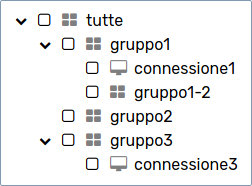
\includegraphics{main/images/tree.png}
\end{center}
\caption{Struttura delle connessioni.}
\label{fig:tree}
\end{figure}

La figura precedente rappresenta un esempio di albero di connessioni.
Sotto la radice \textit{tutte} è possibile notare tre differenti nodi che rappresentano gruppi di connessioni. In genere, i gruppi dell'albero aventi livello di profondità uno delineano ognuno regioni geografiche, mentre quelli di livello due rappresentano le strutture mediche. La maggior parte delle connessioni, quindi, fanno riferimento a struttura e regione ben definite. 

\subsection{Casi d'uso}
\label{sec:casi d'uso}

\begin{center}
\begin{tabular}{c c c c}
\textbf{Operazioni} & \textbf{Super-utente} & \textbf{Amministratore} & \textbf{Utente}\\
\midrule
\textbf{Connessioni}\\
Visualizzazione connessioni & SI & SI & SI\\
Accesso remoto connessioni & SI & SI & SI\\
Aggiunta connessione & SI & Su richiesta & NO\\
Modifica connessione & SI & Su richiesta & NO\\
Eliminazione connessione & SI & Su richiesta & NO\\
\midrule
\textbf{Gruppi}\\
Visualizzazione gruppi & SI & SI & SI\\
Aggiunta gruppo & SI & NO & NO\\
Modifica gruppo & SI & NO & NO\\
Eliminazione gruppo & SI & NO & NO\\
\midrule
Invito utenti & SI & SI & SI\\
Ricerca database & SI & NO & NO\\
Modifica permessi utenti & SI & NO & NO\\
Richiesta comunicazione  & SI & SI & SI
\end{tabular}
\end{center}

Nella tabella sono riportate le operazioni che ciascun livello di utente può eseguire. Alcune di queste sono già state trattate nei paragrafi precedenti, ma in questo caso la tabella risulta utile per avere un quadro completo dei permessi che ciascun utente possiede.
Nel caso delle voci di visualizzazione di connessioni, dei gruppi e di accesso remoto alle connessioni, il valore riferito all'utente base dipende dalle connessioni che gli sono state assegnate al momento dell'invito. Se non viene selezionata alcuna connessione dall'albero, l'utente non potrà accedere e visualizzare alcuna connessione.

\section{Aspetto della piattaforma}
\label{sec:aspetto della piattaforma}

\subsection{Invito utenti}
\label{sec:invito utenti}
Per partecipare alla piattaforma e per poter accedere ai suoi contenuti è necessario effettuare l’iscrizione, che può essere intrapresa solo tramite invito effettuato da un utente già registrato.
La pagina visualizzata al momento dell'apertura della dashboard, dopo aver effettuato il login, è dedicata appunto all'operazione di invito di nuovi utenti. 

\begin{figure}
\begin{center}
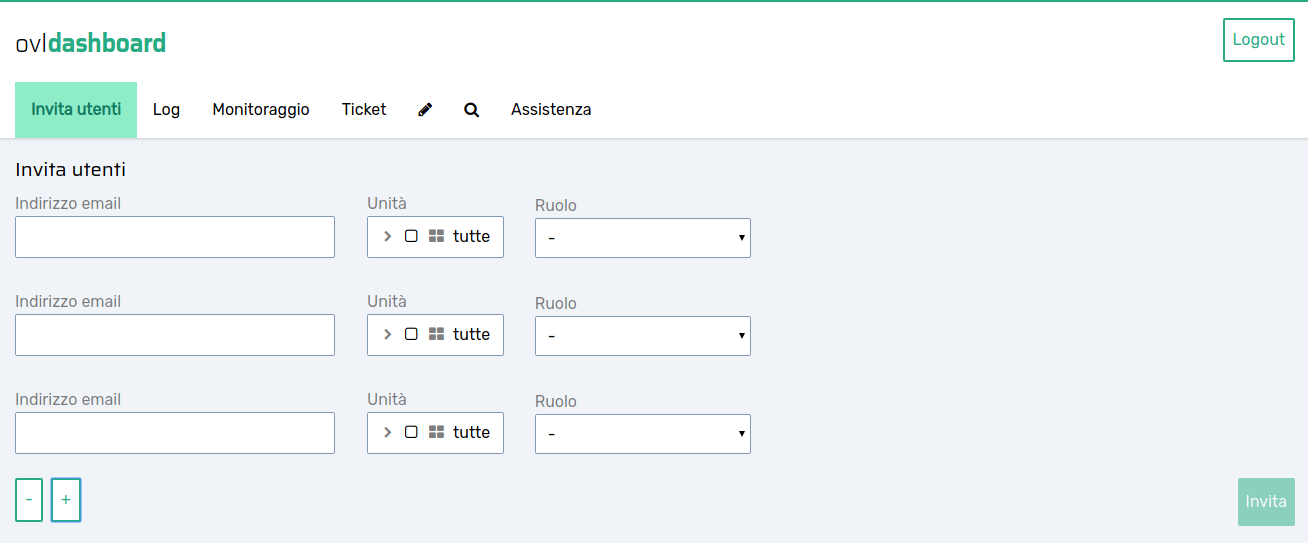
\includegraphics[scale=0.43]{main/images/invitations.png}
\end{center}
\caption{Pagina di invito nuovi utenti.}
\label{fig:invitations}
\end{figure}

La pagina mostra una prima area di input in cui è possibile inserire l'indirizzo e-mail della persona che si desidera invitare ad utilizzare la piattaforma. Successivamente, si indicano le connessioni ed i gruppi a cui il nuovo utente potrà accedere (utilizzando la struttura ad albero precedentemente illustrata) e il ruolo che esso ricopre.
Il numero delle richieste di invito che si desidera effettuare può essere incrementato aggiungendo nuovi form mediante l'apposito tasto.
Procedendo con la conferma verrà inviata una mail (con richiesta al server di autorizzazione) a tutti gli indirizzi precedentemente indicati, ed i rispettivi utenti provvederanno al completamento della registrazione.

Se un invito viene effettuato esplicitando \textit{amministratore} come valore del campo ruolo, il nuovo utente verrà registrato sulla piattaforma con permessi di modifica e eliminazione sulle sole connessioni a cui egli ha accesso.

\subsection{Form connessioni e gruppi}
\label{sec:form connessioni e gruppi}
L'aggiunta di una nuova connessione viene effettuata attraverso un form nel quale l'utente deve specificare caratteristiche e parametri del dispositivo da aggiungere. Tali dati servono al sistema di Guacamole per instaurare la connessione con successo. In particolare, occorre specificare il gruppo a cui la nuova connessione dovrebbe appartenere. 

\begin{figure}
\begin{center}
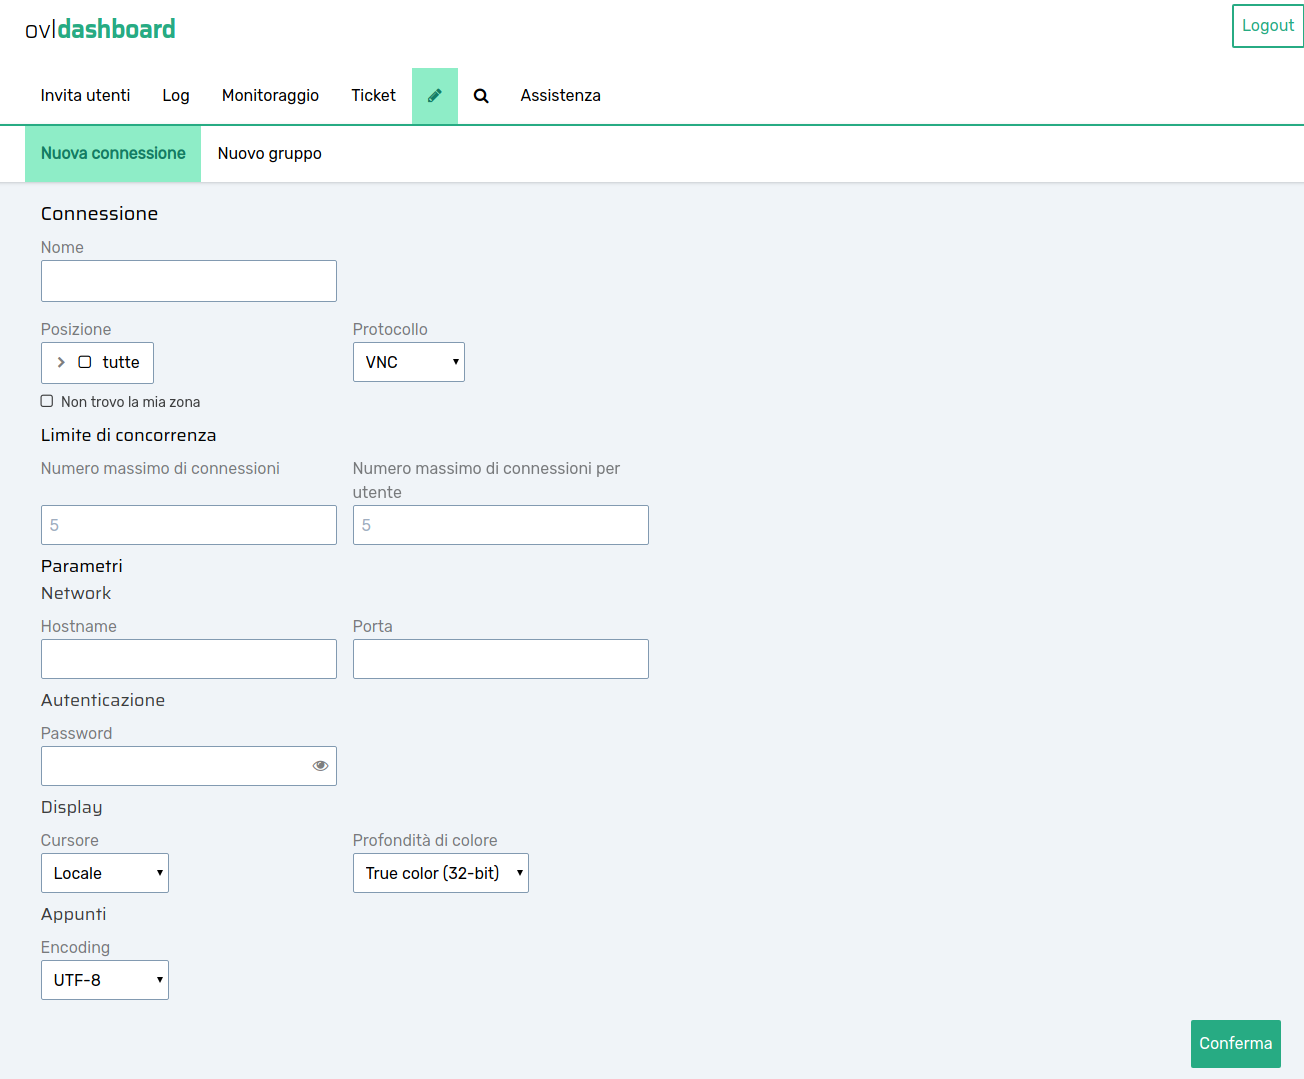
\includegraphics[scale=0.40]{main/images/form.png}
\end{center}
\caption{Form di aggiunta nuova connessione.}
\label{fig:connectionForm}
\end{figure}

L'intera pagina è visibile da tutti gli utenti aventi ruolo amministratore, ma l'inserimento diretto di una nuova connessione nel sistema viene permesso soltanto al super-utente aziendale Themis. 

Al momento della pressione del pulsante di conferma da parte di un utente amministratore, i parametri digitati vengono raccolti ed organizzati sottoforma di richiesta nella pagina \textit{ticket} (questo concetto viene spiegato meglio nella sezione successiva) che verrà approvato o rifiutato in un secondo momento. Se, invece, l'account con cui è stato effettuato il login è quello super-utente, l'azione di conferma crea la nuova connessione fin da subito e sarà disponibile nell'albero e in tutto il sistema.
La differenziazione tra account super-utente e account amministratore è stata mantenuta in ogni caso d'uso riguardante le connessioni: il ticket di richiesta viene creato ogni volta che un utente amministratore ha l'esigenza di aggiungere, modificare o eliminare una connessione sistema. 

Un altro privilegio che possiede l'account super-utente è il fatto di poter visualizzare un altro form dedicato alla gestione dei gruppi avente funzionalità di aggiunta, modifica ed eliminazione parallele a quelle delle connessioni.

Nel caso particolare in cui un utente amministratore deve inserire una connessione per un dispositivo, situato in una località ancora non gestita come gruppo all'interno della piattaforma, può specificare all'interno del form un recapito. Questa informazione permette all'account super-utente di contattare, al momento della gestione del ticket, l'autore della richiesta e, quindi, di aggiungere il gruppo necessario all'inserimento della connessione.

\subsection{Ticket}
\label{sec:ticket}
La pagina dei ticket è strettamente legata alla creazione di nuove connessioni. Questa, infatti, raccoglie tutte le richieste generate dagli utenti amministratori. 
Le richieste vengono generate ogni volta che un utente amministratore desidera aggiungere, modificare o eliminare una connessione. Ogni richiesta viene presentata sottoforma di ticket.

\begin{figure}
\begin{center}
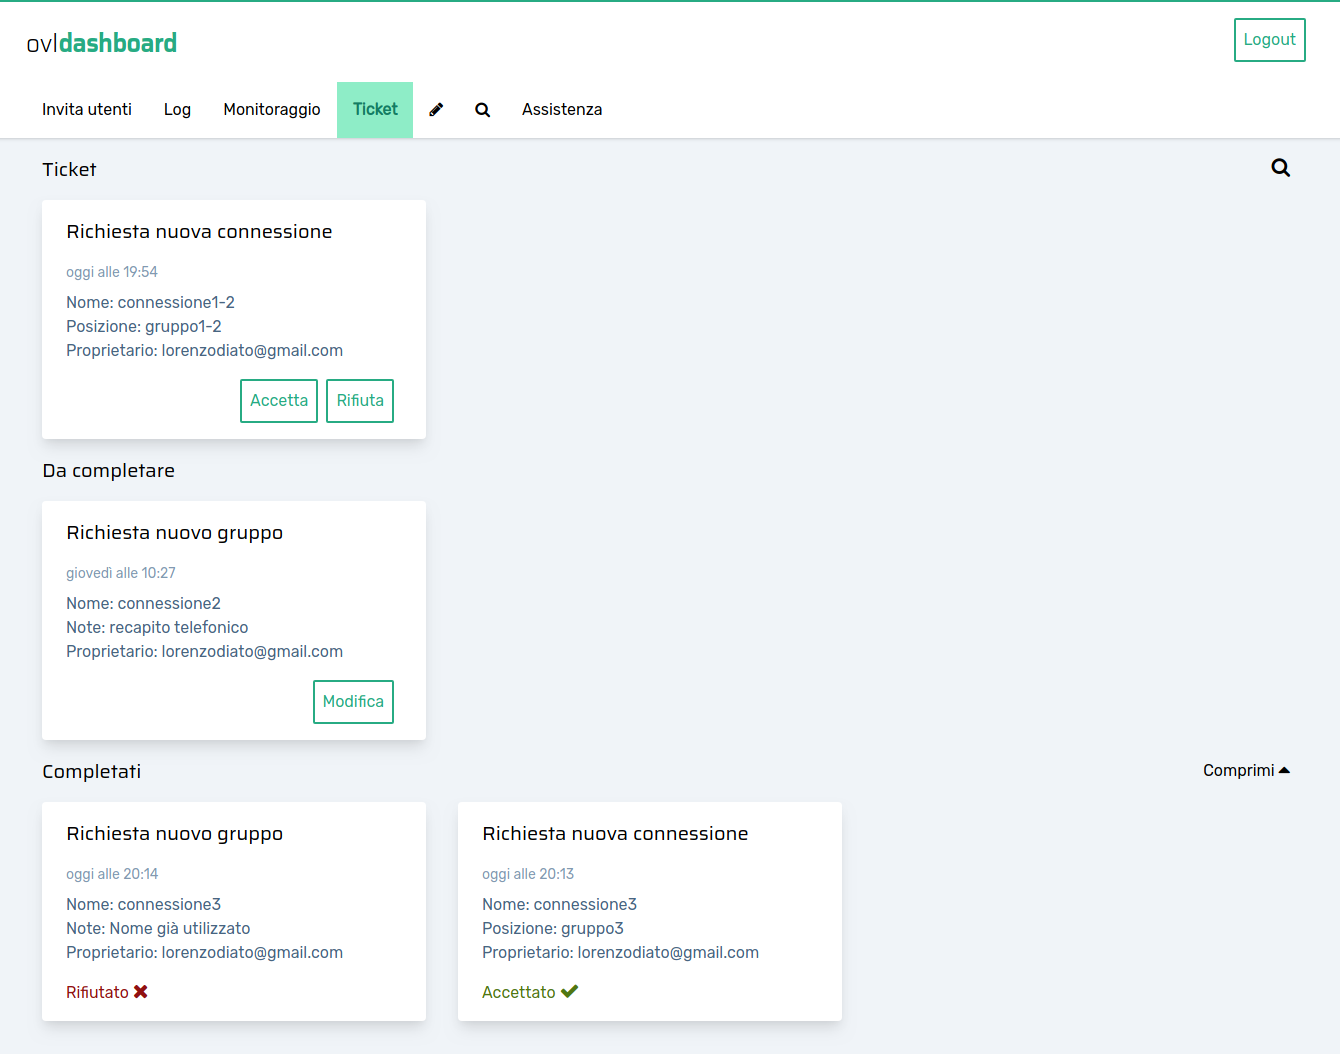
\includegraphics[scale=0.40]{main/images/tickets.png}
\end{center}
\caption{Pagina dei ticket.}
\label{fig:tickets}
\end{figure}

La pagina è suddivisa in tre sezioni: la prima, in alto, mostra i ticket ancora in attesa di riscontro (da accettare o da rifiutare); la seconda, con la dicitura \textit{da completare}, presenta quelli elaborati e presi in carico, ma in attesa di completamento. Infine, l'ultima, in basso, contiene quelli completati e consente di tenere uno storico delle richieste.
Nell'immagine sono presenti due principali tipologie di ticket: le richieste per connessioni di cui si conosce la posizione quindi il gruppo a cui dovrebbe appartenere e le richieste di connessioni il cui gruppo non esiste ancora nell'albero. Nel primo caso, gli utenti che possono risolvere la richiesta, quindi accettarla o rifiutarla sono gli amministratori più importanti dal punto di vista gerarchico e l'account super-utente. Il secondo caso, invece più complesso, può essere gestito solamente dal super-utente che provvede ad aggiungere il gruppo necessario e di conseguenza assegnarlo alla nuova connessione espressa nella richiesta.

In caso di rifiuto della richiesta l'utente deve specificare la motivazione per cui è stata effettuata quella scelta ed eventualmente come risolvere il problema. Le connessioni corrispondenti ai ticket accettati, invece, vengono inserite nel sistema e quindi subito disponibili per il collegamento remoto.

All'interno della pagina è stata implementato un filtro di ricerca: i ticket possono essere organizzati per tipologia, stato corrente o ricercati semplicemente secondo il loro nome.

\subsection{Comunicazione e assistenza}
\label{sec:comunicazione e assistenza}

La porzione di progetto descritta in questo paragrafo è stata progettata da entrambi i componenti del team di sviluppo. Io, in particolare, mi sono occupato del back-end e della creazione di una "demo" funzionante che ha velocizzato l'effettiva implementazione all'interno della dashboard. 

La pagina di assistenza offre all'utente la possibilità di contattare altri utenti mediante chat oppure chiamata vocale. In primo piano viene mostrato l'elenco degli utenti che è possibile contattare suddivisi tra account aventi una sessione attiva e account offline.
Nel caso in cui l'utente che si desidera contattare non fosse online, gli viene inviata un'email che notifica l'avvenuto tentativo di comunicazione e che contiene il collegamento d'accesso alla piattaforma. Quando viene eseguito l'accesso, l'utente viene reindirizzato direttamente alla pagina di assistenza con la comunicazione già inizializzata.